\documentclass[
article, % indica que é um artigo acadêmico
12pt, % tamanho da fonte
oneside, % para impressão apenas no verso. Oposto a twoside
a4paper, % tamanho do papel. 
portuguese, % idioma adicional para hifenização
portuguese % o último idioma é o principal do documento
]{abntex2}
%%%%%%%%%%%%%%%%%%%%%%%%% Credit %%%%%%%%%%%%%%%%%%%%%%%%

% template ini dibuat oleh martin.manullang@if.itera.ac.id untuk dipergunakan oleh seluruh sivitas akademik itera.

%%%%%%%%%%%%%%%%%%%%%%%%% PACKAGE starts HERE %%%%%%%%%%%%%%%%%%%%%%%%
\usepackage{graphicx}
\usepackage[alf]{abntex2cite}
\usepackage{caption}
\usepackage{microtype}
\usepackage{tablefootnote}
%\usepackage{lscape}
\usepackage{pdflscape}
\captionsetup[table]{name=Tabela}
\captionsetup[figure]{name=Figura}
\renewcommand{\figureautorefname}{Figura}
\renewcommand{\tableautorefname}{Tabela}
\renewcommand{\sectionautorefname}{Seção}
\renewcommand{\subsectionautorefname}{Subseção}
\usepackage{tabulary}
\usepackage{minted}
% \usepackage{amsmath}
\usepackage{fancyhdr}
% \usepackage{amssymb}
% \usepackage{amsthm}
\usepackage{placeins}
\usepackage{multicol}
\usepackage{threeparttable}
\usepackage{caption}
\usepackage{colortbl}
\usepackage{subcaption}
% \usepackage{amsfonts}
\usepackage{graphicx}
\usepackage[all]{xy}
\usepackage{tikz}
\usepackage{verbatim}
\usepackage{hyperref}
\usepackage[left=2cm,right=2cm,top=3cm,bottom=2.5cm]{geometry}
\usepackage{hyperref}
\hypersetup{
    colorlinks,
    linkcolor={red!50!black},
    citecolor={blue!50!black},
    urlcolor={blue!80!black}
}
\usepackage{caption}
\usepackage{subcaption}
\usepackage{multirow}
\usepackage{psfrag}
\usepackage[T1]{fontenc}
\usepackage[scaled]{beramono}
% Enable inserting code into the document
\usepackage{listings}
\usepackage{xcolor} 
% custom color & style for listing
\definecolor{codegreen}{rgb}{0,0.6,0}
\definecolor{codegray}{rgb}{0.5,0.5,0.5}
\definecolor{codepurple}{rgb}{0.58,0,0.82}
\definecolor{backcolour}{rgb}{0.95,0.95,0.92}
\definecolor{LightGray}{gray}{0.9}
\lstdefinestyle{mystyle}{
	backgroundcolor=\color{backcolour},   
	commentstyle=\color{green},
	keywordstyle=\color{codegreen},
	numberstyle=\tiny\color{codegray},
	stringstyle=\color{codepurple},
	basicstyle=\ttfamily\footnotesize,
	breakatwhitespace=false,         
	breaklines=true,                 
	captionpos=b,                    
	keepspaces=true,                 
	numbers=left,                    
	numbersep=5pt,                  
	showspaces=false,                
	showstringspaces=false,
	showtabs=false,                  
	tabsize=2
}
\lstset{style=mystyle}
\renewcommand{\lstlistingname}{Kode}
%%%%%%%%%%%%%%%%%%%%%%%%% PACKAGE ends HERE %%%%%%%%%%%%%%%%%%%%%%%%


%%%%%%%%%%%%%%%%%%%%%%%%% Data Diri %%%%%%%%%%%%%%%%%%%%%%%%
%\newcommand{\student}{\textbf{Isi Nama Di Sini (Dan Nim Di Sini)}}
%\newcommand{\course}{\textbf{Nama Mata Kuliah (Kode Mata Kuliah)}}
%\newcommand{\assignment}{\textbf{xxx}}

%%%%%%%%%%%%%%%%%%% using theorem style %%%%%%%%%%%%%%%%%%%%
\newtheorem{thm}{Theorem}
\newtheorem{lem}[thm]{Lemma}
\newtheorem{defn}[thm]{Definition}
\newtheorem{exa}[thm]{Example}
\newtheorem{rem}[thm]{Remark}
\newtheorem{coro}[thm]{Corollary}
\newtheorem{quest}{Question}[section]
%%%%%%%%%%%%%%%%%%%%%%%%%%%%%%%%%%%%%%%%
\usepackage{lipsum}%% a garbage package you don't need except to create examples.
\usepackage{fancyhdr}
\pagestyle{fancy}
\lhead{Pedro Jorge Holanda Alves}
\rhead{ \thepage}
\cfoot{\textbf{Processo seletivo 4i}}
\renewcommand{\headrulewidth}{0.4pt}
\renewcommand{\footrulewidth}{0.4pt}

%%%%%%%%%%%%%%  Shortcut for usual set of numbers  %%%%%%%%%%%

\newcommand{\N}{\mathbb{N}}
\newcommand{\Z}{\mathbb{Z}}
\newcommand{\Q}{\mathbb{Q}}
\newcommand{\R}{\mathbb{R}}
\newcommand{\C}{\mathbb{C}}
\setlength\headheight{14pt}

%%%%%%%%%%%%%%%%%%%%%%%%%%%%%%%%%%%%%%%%%%%%%%%%%%%%%%%555
\begin{document}
\thispagestyle{empty}
%\begin{center}
%	\includegraphics[scale = 0.4]{Figure/ifitera-header.jpg}
%	\vspace{0.1cm}
%\end{center}
\noindent
\rule{17cm}{0.2cm}\\[0.3cm]
Nome:  Pedro Jorge Holanda Alves \hfill \href{https://github.com/PedroJorge7/Processo4i}{Script com código em R}\\[0.1cm]
Processo Seletivo 4i \\
\rule{17cm}{0.05cm}
\vspace{0.1cm}



%%%%%%%%%%%%%%%%%%%%%%%%%%%%%%%%%%%%%%%%%%%%% BODY DOCUMENT %%%%%%%%%%%%%%%%%%%%%%%%%%%%%%%%%%%%%%%%%%%%%




\section{Exercício de conjuntura econômica}

O processo de globalização nos últimos 20 anos permitiu que os países possam cada vez mais realizar trocas rápidas e eficientes, causando um efeito deflacionário. No entanto, a ocorrência de choques externos, como a COVID-19 e novas tensões geopolíticas fazem com que as cadeias produtivas não sejam implantadas de forma eficiente e que os fluxos de comércio sejam mais difíceis, o que gera um efeito inflacionário.

A guerra entre Rússia e Ucrânia é um exemplo de como um choque pode impactar indiretamente a economia de um país. Como mostra a \autoref{tab:01}, tanto a Rússia, como a Ucrânia, possuem participações pequenas no agregado mundial, representando 1,75\% e 0,17\% do Produto Interno Bruto (PIB) mundial, respectivamente. Mesmo que seus pesos sob o resto do mundo sejam pequenos, seus acordos comerciais podem afetar outros países de forma indireta, acarretando perdas no poder econômico desses países parceiros.

\begin{table}[H] 
  \centering
  \caption{Descrições gerais: Rússia e Ucrânia (2020)}
    \begin{tabular}{l|cccc}
    \hline
    Indicadores & Rússia & \% no mundo & Ucrânia & \% no mundo \\
    \hline
    GDP (Trilhões) & 1,48  & 1,75  & 0,16  & 0,18 \\
    População (Milhões) & 144,10 & 1,86  & 44,13 & 0,57 \\
    Exportação (Bilhões) & 378,64 & 1,69  & 60,74 & 0,27 \\
    Importação (Bilhões) & 305,01 & 1,40  & 62,38 & 0,29 \\
    \hline
    \multicolumn{4}{l}{Fonte: World bank. Elaboração própria.}
    \end{tabular}%
  \label{tab:01}%
\end{table}%

De acordo com os dados \textit{World Integrated Trade Solution} (Wits)/Comtrade \footnote{Disponível em: \href{https://wits.worldbank.org/}{https://wits.worldbank.org/}. Acesso em: 25 abr. 2022}, a Rússia possuía em 2018 cerca de 224 parceiros de importação e 198 de exportação, enquanto que a Ucrânia tinha 202 e 193, respectivamente. A Rússia é um país extremamente importante na produção de diversas \textit{commodities} e também é um grande ofertante de energia para a Europa (38\% do gás, 29\% do petróleo e 50\% do carvão importado pela Europa). A Ucrânia possui grande relevância na comercialização de alguns produtos agrícolas, como girassol, milho e trigo. A interrupção de seu fornecimento ocasiona uma rápida mudança nos preços.


\subsection{QUESTÃO 1}

Os países que vão sentir mais impacto com essa crise são aqueles que são mais vulneráveis a choques eternos (muito dependentes do mercado internacional, principalmente da Rússia ou Ucrânia). Para que seja possível avaliar os impactos indiretos da guerra entre a Rússia e Ucrânia foi utilizado os dados do (Wits)/Comtrade com o auxílio na nota técnica do IPEA, elaborada por \citeonline{Nonnenberg2022}. As informações foram coletadas de acordo com último ano disponível para cada país (2020, Rússia e 2021, Ucrânia). Neste momento, é difícil fazer qualquer afirmação sobre todos os efeitos da guerra e seus desdobramentos. Contudo, a partir dos levantamentos sobre quais os bens que cada país exporta e importa é possível discutir de que forma o mundo e o Brasil poderão ser afetados.

%Quais canais o comércio internacional seria mais afetado pela guerra? Com o inicio da guerra, tanto a Ucrânia será afetada com a interrupção na produção, exportação e importação. Mesmo que a Rússia não sofra com a mesma magnitude (por não ser o território de guerra), sua atividade econômica também sofrerá perda. Boa parte dos países europeus e o Estados Unidos também aplicaram restrições financeiras, comerciais e bancárias capazes de afetar as exportações e importações da Rússia. Todos esses efeitos se somarão junto aos efeitos da pandemia da Covid-19 e irá, de forma inevitável, elevar os preços. Quanto mais tempo durar o conflito e quanto mais severas forem as suas consequências.

%De 1º  de fevereiro até 3 de março, os preços do barril de petróleo Brent subiram 26,5\%; os do trigo, 47,4\%; e os do milho, 19,1\%. Isso afeta todos os países exportadores e importadores. A redução da demanda e a recessão nesses três países também terão efeitos sobre os demais.

% Para compreender de forma mais clara os efeitos da guerra, foi levantado informações estatísticas sobre os dois países e quais os potenciais efeitos para os países parceiros. A \autoref{fig:01} apresenta o percentual de participação de cada país nas exportações e importações da Rússia em 2020. Os dados foram retirados da \textit{World Integrated Trade Solution} (Wits)/Comtrade.

A partir da visualização do mapa, é possível verificar que a China tem maior de participação das exportações (25\%) e importações (16\%) da Rússia, seguido de Alemanha e Grã betanha (10\% e 7,5\% das exportações) e Países baixos (8\% das importações). O Brasil vem logo em seguida, participando de 5,6\% das importações da Rússia e 4,5\% das exportações Por outro lado, países do continente Africano e os restantes dos países da América do Sul tiveram participação baixa no comércio com a Rússia (menos de 1\%). Os Estados Unidos, mesmo que não esteja entre os maiores, aparece com 4,11\% e 3,4\% das importações e exportações, respectivamente.

\begin{figure}[H]
    \centering
    \caption{Participação nas exportações e importações da Rússia}
    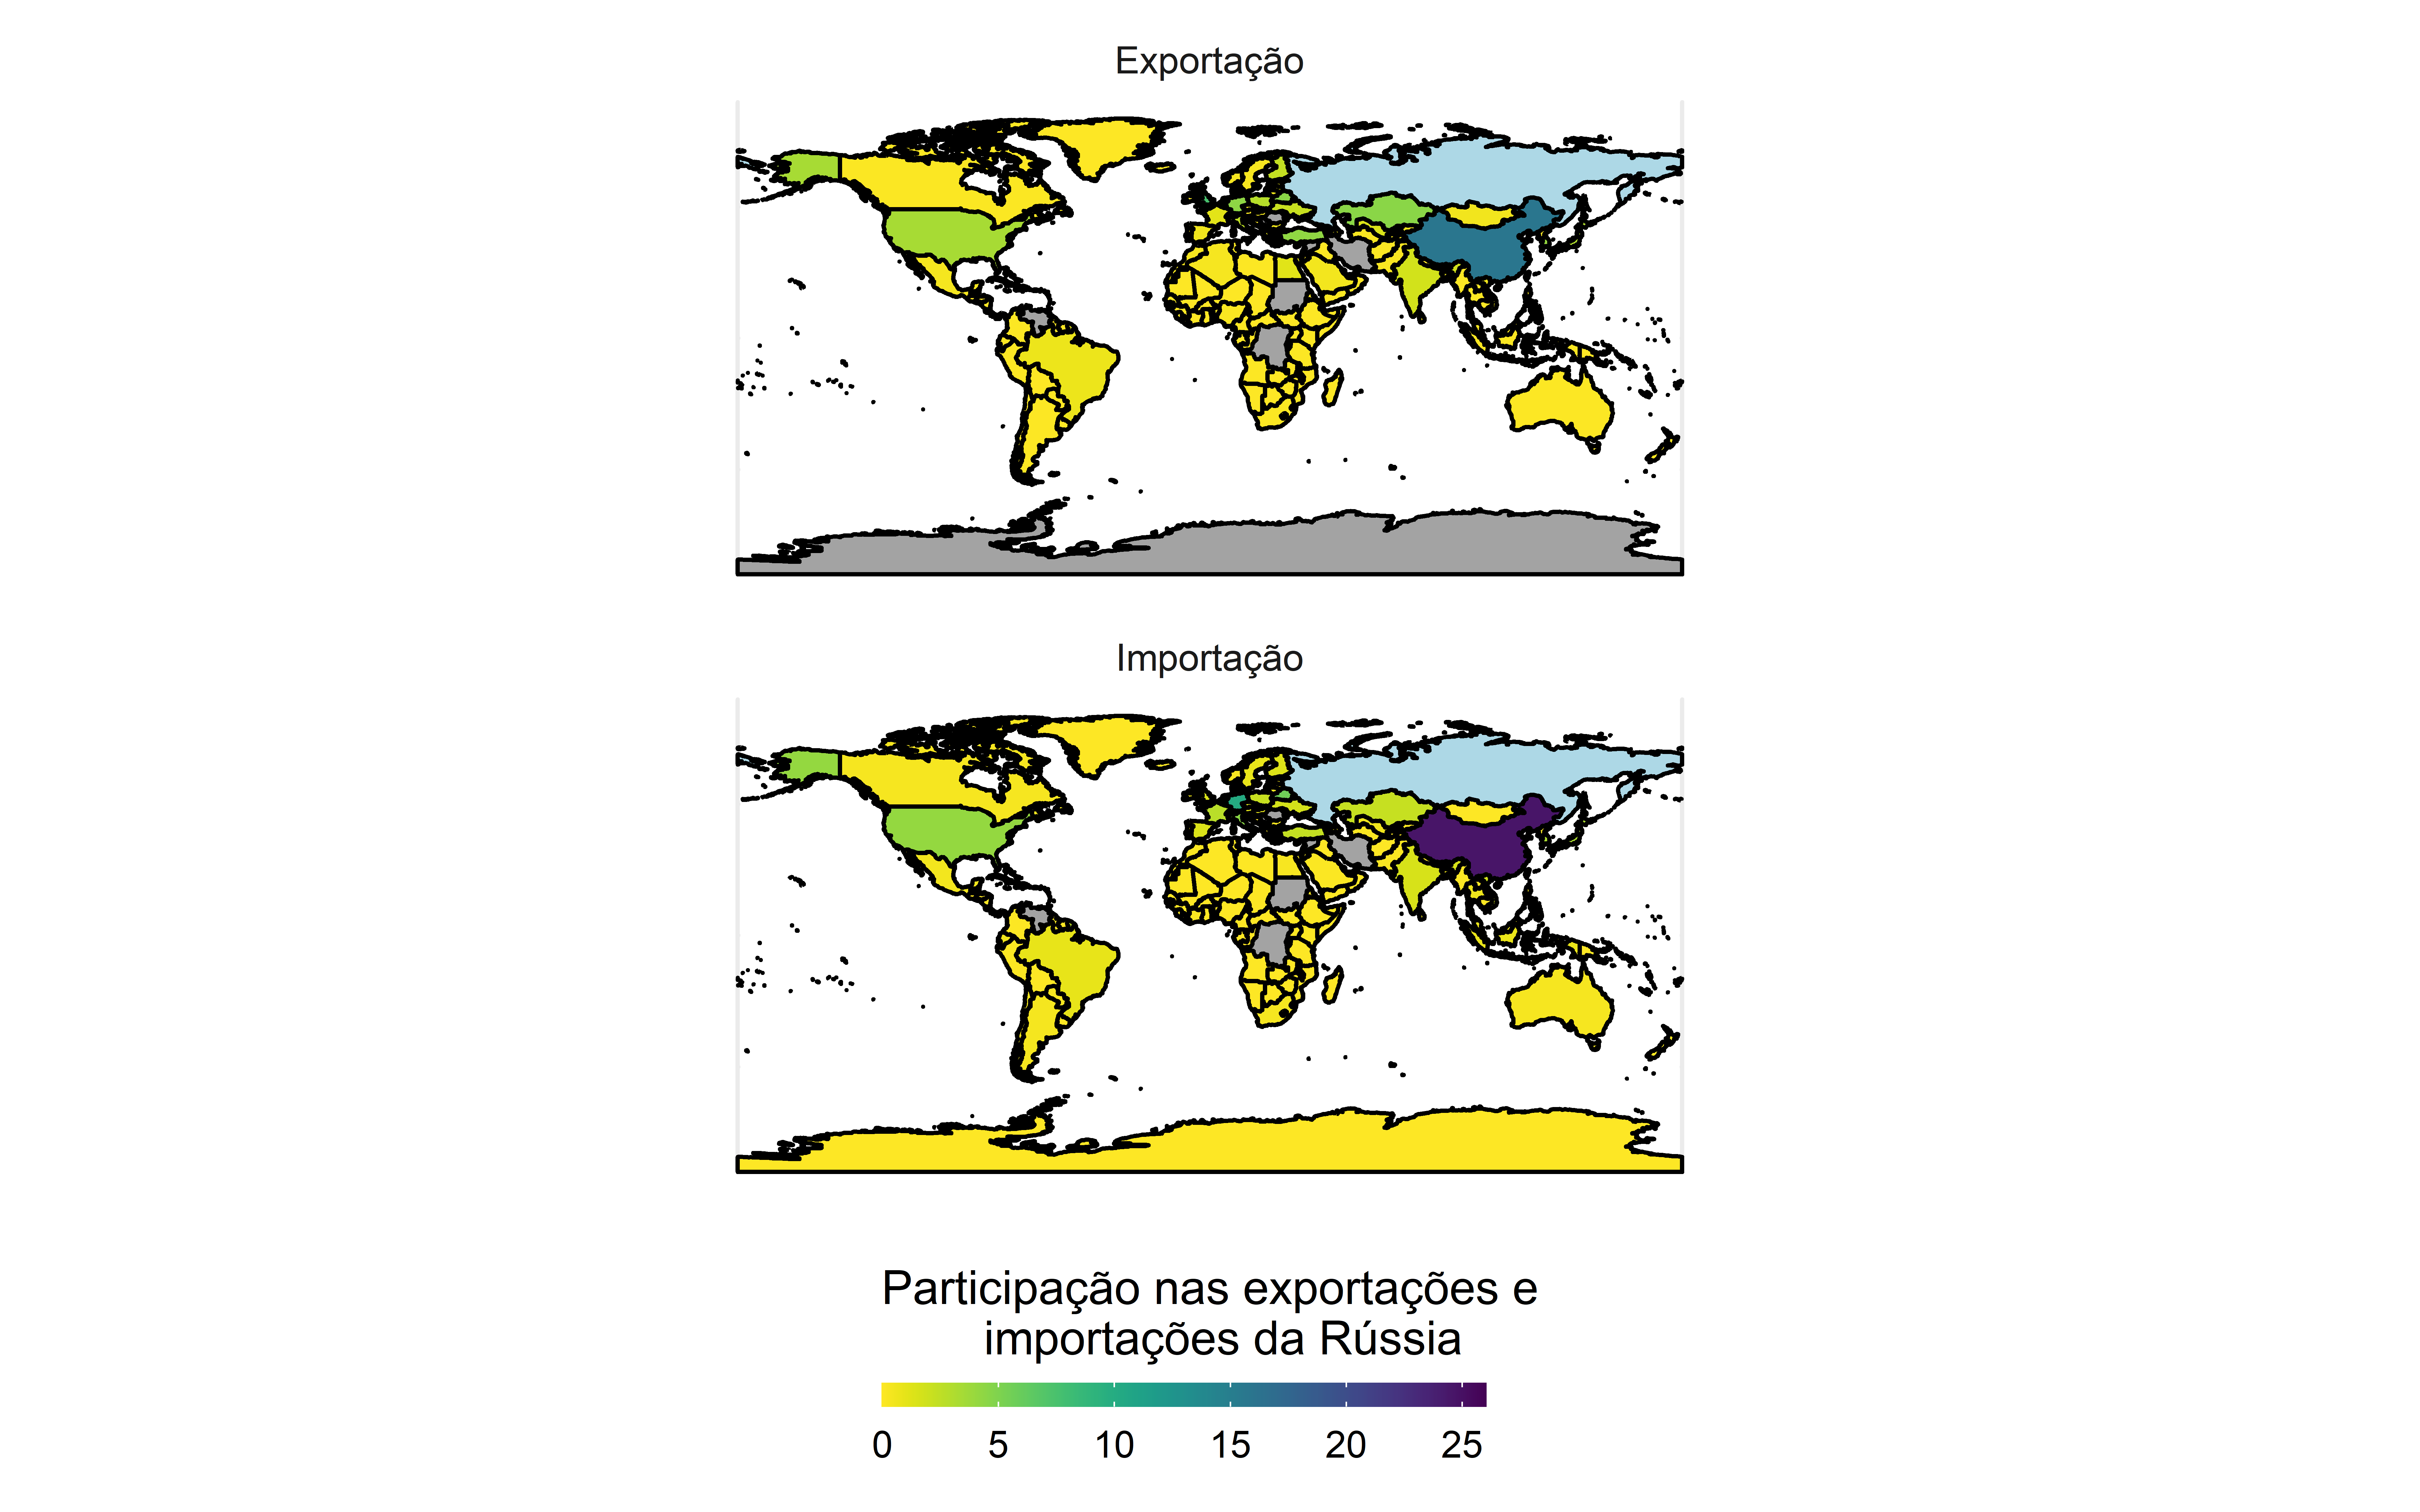
\includegraphics[width=1\textwidth]{figuras/Participação nas exportações e importações da Rússia.png}
    \begin{flushleft}
    Fonte: Wits/Comtrade. Elaboração própria.
    \end{flushleft}
    \label{fig:01}
\end{figure}

A participação das exportações mundiais da Ucrânia é ainda menor, representando cerca de 0,1\% das exportações mundiais. Dentre os países que a Ucrânia mais exporta, se destacam a China (12,2\%), Polônia (7,6\%), Turquia(6\%) e Itália (4,9\%). O Brasil aparece possui 2,2\% das exportações da Ucrânia. No sentido das importações, o país tem China (12,3\%), Alemanha (8,7\%), Rússia (8,4\%), Polônia (7\%) e Brasil (6,8\%) como países que mais depende de importações. Os Estados Unidos representa 4,8\% das importações da Ucrânia e 2,34\% das exportações.

Assim como na Rússia, países do continente Africano e os outros países da América do Sul possuem baixa participação na balança comercial da Ucrânia. Por outro lado, a China, Estados Unidos e os países da Europa acabam sendo afetados pela falta de abastecimento tanto na questão de exportar para a Rússia ou Ucrânia, como também de importar produtos desses países (falta de insumo). No caso dos países da Europa, por exemplo, a Rússia é um grande abastecedor de energia e a falta de fornecimento pode gerar grandes implicações na economia da região.

\begin{figure}[H]
    \centering
    \caption{Participação nas exportações e importações da Ucrânia}
    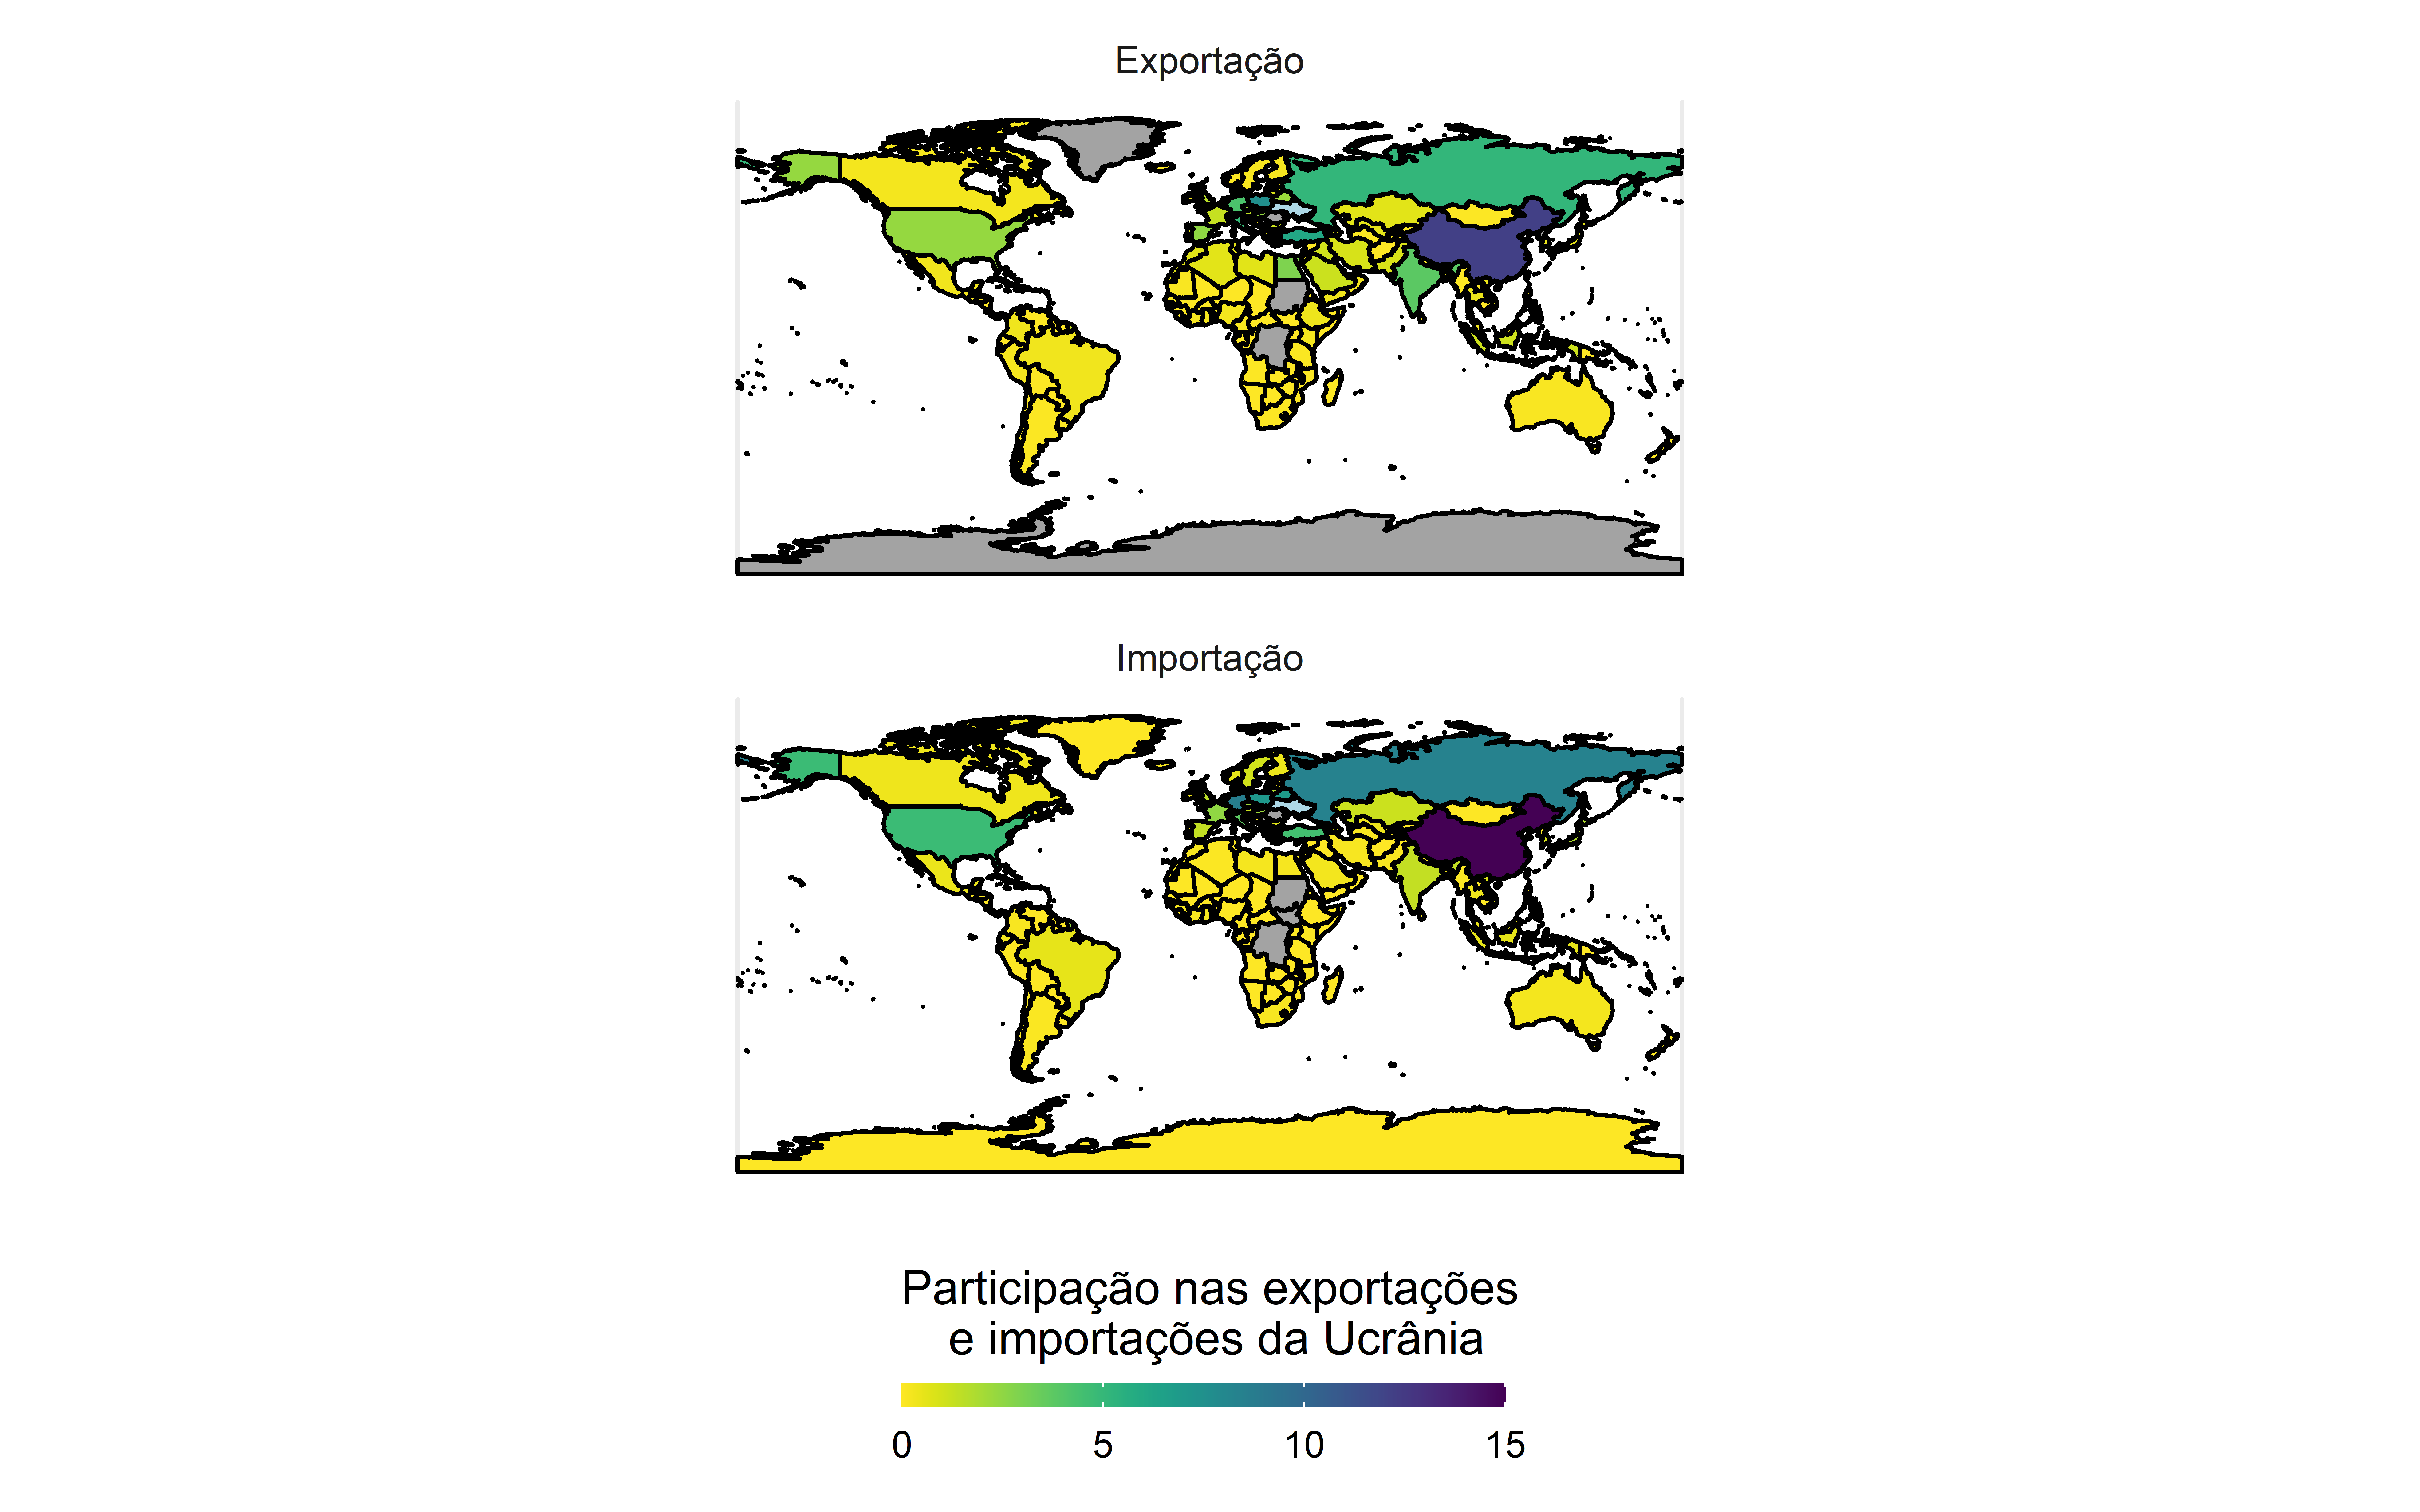
\includegraphics[width=1\textwidth]{figuras/Participação nas exportações e importações da Ucrânia.png}
    \begin{flushleft}
    Fonte: Wits/Comtrade. Elaboração própria.
    \end{flushleft}
    \label{fig:02}
\end{figure}

O próximo passo é examinar com mais detalhes os principais produtos potencialmente afetados devido a guerra. \autoref{tab02} aponta os principais produtos exportados pela Rússia e Ucrânia, o valor apresentado, a participação no total de exportações e os principais mercados abastecidos. A Rússia em 2020 exportou principalmente o Petróleo Bruto (representando 24\% das suas exportações no ano), Petróleo Refinado (15\%), Alumínio (6\%), Hulhas (4\%) e Trigo (2,7\%). Desses produtos, China, Holanda e Alemanha são grandes importadores de petróleo bruto e Holanda, Estados Unidos, Turquia e Alemanha são os principais importadores do petróleo refinado. O alumínio teve 91\% das exportações com destino ao Reino Unido.

A Ucrânia em 2021 teve o minério de ferro como o produto mais exportado (10,4\%), seguido de óleo de girassol (9,6\%), milho (8,9\%), trigo (7,2\%) e semimanufaturado de ferro (6\%). Os maiores importadores de minério de ferro Ucrânia foram a China (43\%), República Checa (10\%) e Áustria (8\%). Em relação ao óleo de girassol a Índia aparece como a maior importadora com 30\%, seguido da China (15\%) e Holanda (10\%).

\begin{landscape} 
\begin{table}[H] 
\caption{Principais produtos exportados pela Rússia e Ucrânia e seus parceiros comerciais} \label{tab02}

\begin{tabular}{l|c|c|m{20em}}
\hline
\multicolumn{1}{m{13em}|}{Principais produtos exportados} & \multicolumn{1}{m{10em}|}{Valor das exportações
(em milhões de US\$)} & \multicolumn{1}{m{7em}|}{\% do total exportado} & Principais países que exporta\\
\hline
\multicolumn{4}{l}{\textbf{Rússia (2020)}}\\
\hline
\hspace{1em}Petróleo Bruto & 72,56 & 24,37 & China (33\%), Holanda (13\%), Alemanha (9\%), Coreia (7\%), Polônia (6\%)\\
\hline
\hspace{1em}Petróleo Refinado & 45,36 & 15,23 & Holanda (15\%), Estados Unidos (10\%), Turquia (5\%), Alemanha (5\%), China (5\%)\\
\hline
\hspace{1em}Alumínio & 18,54 & 6,22 & Reino Unido (91\%), Suiça (3\%), Cazaquistão (2\%), Turquia (2\%), Índia (1\%)\\
\hline
\hspace{1em}Hulhas & 12,39 & 4,16 & China (15\%), Coreia do Sul (13\%), Japão (12\%), Turquia (7\%), Outros países da Ásia (5\%) \\
\hline
\hspace{1em}Trigo & 7,92 & 2,66 & Egito (23\%), Turquia (21\%), Bangladesh (5\%), Azerbaijão (4\%), Sudão (4\%)\\
\hline
\multicolumn{4}{l}{\textbf{Ucrânia (2021)}}\\
\hline
\hspace{1em}Minério de ferro & 6,81 & 10,38 & China (43\%), República Tcheca (10\%), Áustria (8\%), Polônia (8\%), Eslováquia (6\%)\\
\hline
\hspace{1em}Óleo de girassol & 6.31 & 9.62 & Índia (30\%), China (15\%), Holanda (10\%), Espanha (7\%), Itália (5\%)\\
\hline
\hspace{1em}Milho & 5,85 & 8,92 & China (32\%), Espanha (10\%), Holanda (9\%), Egito (9\%), Irã-Islã (7\%)\\
\hline
\hspace{1em}Trigo & 4.72 & 7.20 & Egito (18\%), Indonésia (14\%), Turquia (8\%), Paquistão (7\%), Marrocos (6\%)\\
\hline
\hspace{1em}Semimanufaturados de ferro & 3.89 & 5.92 & Itália (30\%), Turquia (13\%), República Dominicana (8\%), Bulgária (7\%), China (5\%)\\
\hline
\multicolumn{4}{l}{Fonte: Wits/Comtrade. Elaboração própria.}
\end{tabular}
\end{table}
\end{landscape} 

Em relação aos principais produtos importados, a \autoref{tab02} mostra que a Rússia em 2020 importou principalmente aparelhos transmissores (3,8\% do total da importação do país), Acessório de veículo (3,4\%), Medicamentos (3,2\%), Motor de veículo (2,4\%) e Máquinas automáticas (2,2\%). Do total de aparelhos transmissores importados, 71\% teve origem da China, 15\% do Vietnã e 3\% da Índia. Já os acessório de veículos teve 16\% de origem alemã, 15\% Coreia 14\%, Japão 13\%.

A Ucrânia teve o Petróleo Refinado como principal produto importado, com 7,8\% e Belarus (42\%), Rússia (23\%), Lituânia (11\%) como os principais produtores fornecedores. Motor de veículo foi o segundo produto mais importado, com 6,3\% das importações do pais, originado principalmente dos Estados Unidos (19\%), Japão (17\%) e Alemanha (16\%). Os outros produtos mais importados foram Gás de petróleo (4,2\%), Hulhas (3,5\%) e Medicamentos (3,1\%).

A falta de abastecimento com os bens importados dos países envolvidos na guerra podem resultar na queda em algumas carteiras no mercado de ações que estejam relacionadas a esses bens. Por exemplo, um país dependente de insumo agrícola da Rússia pode sofrer negativamente na atividade econômica de \textit{commodities} e também no mercado acionário que tenha envolvimento com este meio de produção. Assim, a guerra pode afetar negativamente não só os países envolvidos, mas também os países que são parceiros comerciais dos mesmos. A falta de importação de algum produto pode acarretar na estagnação da produção de algum produto.

\begin{landscape}  
\begin{table}[H]

\caption{Principais produtos importados pela Rússia e Ucrânia e seus parceiros comerciais} \label{tab03}

\begin{tabular}{l|c|c|m{20em}}
\hline
\multicolumn{1}{m{13em}|}{Principais produtos importados} & \multicolumn{1}{m{10em}|}{Valor das importações
(em milhões de US\$)} & \multicolumn{1}{m{7em}|}{\% do total importado} & Principais países que importa\\
\hline
\multicolumn{4}{l}{\textbf{Rússia (2020)}}\\
\hline
\hspace{1em}Aparelhos transmissores & 8,55 & 3,84 & China (71\%), Vietnã (15\%), Índia (3\%), República Tcheca (1\%), Outros países da Ásia (1\% )\\
\hline
\hspace{1em}Acessório de veículo & 7.65 & 3.44 & Alemanha (16\%), China (15\%), Coreia do Sul (14\%), Japão (13\%), República Tcheca (7\%) \\
\hline
\hspace{1em}Medicamentos & 7.21 & 3.24 & Alemanha (20\%), Itália (9\%), Estados Unidos (8\%), Índia (7\%), Suiça (7\%)\\
\hline
\hspace{1em}Motor de veiculo & 5.43 & 2.44 & Japão (24\%), Estados Unidos (17\%), Alemanha (15\%), Eslováquia (8\%), Reino Unido (7\%) \\
\hline
\hspace{1em}Máquinas automáticas & 4.85 & 2.18 & China (73\%), República Tcheca (6\%), Polônia (6\%), Hungria (3\%), Outros países da Ásia (2\%) \\
\hline
\multicolumn{4}{l}{\textbf{Ucrânia (2021)}}\\
\hline
\hspace{1em}Petróleo Refinado & 5.44 & 7.81 & Belarus (42\%), Rússia (23\%), Lituânia (11\%), Turquia (4\%), Grécia (3\%)\\
\hline
\hspace{1em}Motor de veiculo & 4.39 & 6.29 & Estados Unidos (19\%), Japão (17\%), Alemanha (16\%), Polônia (5\%), Hungria (5\%)\\
\hline
\hspace{1em}Gás de petróleo & 2,94 & 4,21 & Suíça (35\%), Rússia (12\%), Cazaquistão (10\%), República Tcheca (7\%), Bielorrússia (6\% )\\
\hline
\hspace{1em}Hulhas & 2,40 & 3,45 & Rússia (61\%), Estados Unidos (21\%), Cazaquistão (10\%), Austrália (4\%), Polônia (3\%)\\
\hline
\hspace{1em}Medicamentos & 2.13 & 3.06 & Alemanha (21\%), Índia (11\%), Itália (8\%), França (7\%), Eslovênia (6\%)\\
\hline
\multicolumn{4}{l}{Fonte: Wits/Comtrade. Elaboração própria.}
\end{tabular}
\end{table}
\end{landscape}  

No geral, os dados mostram que mesmo que a Ucrânia e Rússia tivessem baixos percentuais dentro do PIB global, é possível que a guerra realizada entre ambos afetem grandes economias. A China, países europeus e os Estados Unidos são afetados pela Rússia por problemas no fornecimento de energia. Do lado da Ucrânia, os países sofrem pela falta de fornecimento de produtos agrícolas. Em relação a importação de bens, tanto a Rússia, como a Ucrânia afetam a China, Estados Unidos e os países europeus com a falta de compra de produtos eletrônicos, mecânicos e medicamentos.

As restrições de mercado, causadas pela guerra, também podem afetar a economia de outra forma. Os conflitos, além de afetar a cadeira produtiva do país, também causa fuga de capitais e efeitos negativos no mercado financeiro, devido a insegurança gerada pelo conflito \cite{schneider2006war,brune2015war}. Dessa forma, alguns países podem se beneficiar com a entrada de novo capital estrangeiro (que esteja fugindo da Ucrânia ou Rússia).




\subsection{QUESTÃO 2}

A guerra entre Rússia e Ucrânia pode impactar o Brasil não apenas devido às barreiras internacionais aplicadas à Rússia, mas também em razão de todos os efeitos causados a toda a logística global decorrentes da guerra. A \autoref{fig:03} e a \autoref{fig:04} apresentam as cinco principais mercadorias que o Brasil importou e exportou para a Rússia e Ucrânia em 2021. Para o levantamento dessas informações, foi utilizado os dados provenientes do Comex stat, portal do Ministério da Indústria, Comércio Exterior e Serviços (MDIC) para acesso das estatísticas de comércio exterior do Brasil. 

No ano de 2021, o Brasil teve uma balança comercial positiva de R\$ 61 bilhões, exportando R\$ 280 bilhões e importando R\$ 219 bilhões. Somando todos os acordos comerciais realizados entre o Brasil e a Rússia, o país apresenta uma balança comercial deficitária de -R\$ 4,1 bilhões. Do total exportado e importado, cerca de 0,56\% das exportações brasileiras tiveram a Rússia como destino, enquanto que 2,6\% das importações do país vieram da Rússia.

A \autoref{fig:03} destaca as mercadorias com os maiores valores exportados e importados da Rússia (os valores dentro de cada barra representam o percentual de cada produto no total de cada mercadoria). Dentre os produtos exportados, o Brasil tem grande parte de suas mercadorias destacada por \textit{commodities}, mas com proporção baixa de destinação para Rússia (com exceção do Amendoim, que teve 39\% de seu total importado pela Rússia).

Por outro lado, o volume de produto importado da Rússia é maior, com destaque dos cloretos de potássio (R\$ 1,3 bilhões), Diidrogeno-ortofosfato de amônio (R\$ 0,8 bilhões), Ureia\footnote{Composto orgânico cristalino} (R\$ 0,5 bilhões), Hulha betuminosa\footnote{Carvão que contém uma substância semelhante ao asfalto} (R\$ 0,4 bilhões) e Nitrato de Amônio (R\$ 0,37 bilhões). Todos esses valores importados são maiores que o produto que o Brasil mais exportou para a Rússia (Soja retornou R\$ 0,34 bilhões de exportações para a Rússia). Além de ter importado mais, o Brasil apresenta maior percentual de dependência desses produtos. No caso do Nitrato, por exemplo, 98\% das importações são da Rússia. Outros casos também apresentam proporções elevadas, como outros cloretos de potássio (33\%) e diidrogeno-ortofosfato de amônio (30\%).

\begin{figure}
    \centering
    \caption{Produtos importados da Rússia}
    \includegraphics[width=0.8\textwidth]{figuras/importados da Rússia.png}
    \begin{flushleft}
    Fonte: Comex stat. Elaboração própria.
    \end{flushleft}
    \label{fig:03}
\end{figure}

No caso do comércio com a Ucrânia, o Brasil teve \textit{superavit} comercial de R\$ 15,4 milhões, exportando \textit{commodities} e importando mercadoria bem diversificada, variando entre medicamentos, produtos elétricos e laminados planos de ferro ou aço. Em comparação com a Rússia, o valor de acordos comerciais é menor. Na \autoref{fig:04} é possível verificar que dentre os cinco produtos mais exportados do Brasil para a Ucrânia, os amendoins representavam cerva de 9\% do total exportado do produto e a Bauxita 17\%. Do lado das importações, os Billets de ferro tinham 59\% das compras oriundas da Ucrânia. Outros produtos laminados planos (20\%) e medicamentos que contenham insulina (49\%) também tiveram proporções elevadas.


%O primeiro efeito da guerra ocorreu na parte energética da Europa, que tem grande influência dos produtos Russos. A falta de abastecimento gera consequência de um aumento da  inflação na Europa e elevação da taxa de juros. Ainda se recuperando da pandemia, os países também apresentam fragilidades. 


% mas, de certa forma, isso pode representar, também, um problema para o abastecimento interno, com pressões inflacionárias sobre os preços dos alimentos, que já apresentam tendência de alta no mercado nacional (gráfico 1). Vale lembrar que o preço do milho é decisivo para a formação dos preços de carnes de suínos e frangos


%2º parte - pandemia (inflação crescendo no mundo inteiro)
%3º parte - fertilizantes (25\% deles é do Brasil). Tem um custo enorme na produção de produtos agrícolas. Alta de preço de alimentos
%4º parte - Restringir exportações de grãos

%A grande bola da vez -> segurança alimentar. alta de preço de alimentos

%Vantagem comparativa -> outros países já vão ocupar o lugar da Rússia

%Desasbastecimento interno -> Isso seria em menor escala. Na verdade, quando um país já exporta muito daquilo e um concorrente para, os produtores locais vão se preparar para exportar mais. No inicio o preço pode se elevar, mas depois os produtores vão se antecipar e produzir mais

%Investimentos estrangeiros. Brasil como é um país emergente (BRICS) recebe muito investimento na bolsa por causa disso (uma das coisas para o dolar cair, além da queda da taxa de juros). Justamente o desejo dos investidores de procurar o mercado emergenete


\begin{figure}[H]
    \centering
    \caption{Produtos importados da Ucrânia}
    \includegraphics[width=0.8\textwidth]{figuras/importados da Ucrânia.png}
    \begin{flushleft}
    Fonte: Comex stat. Elaboração própria.
    \end{flushleft}
    \label{fig:04}
\end{figure}

No geral, é possível afirmar que o Brasil pode ser afetado por falta de abastecimento dos produtos importados da Rússia e Ucrânia, visto que alguns produtos são em grande parte oriundos desses países. O Brasil também apresenta grande participação nas importações de fertilizantes vindo da Rússia (cerca de 25\%). A escassez desse produto pode elevar o custo na produção de produtos agrícolas, o que acarreta em uma alta no preço de alimentos. O setor automobilístico também acaba sendo afetado, já que a Rússia é um grande fornecedor do paládio e o material é um insumo importante para a fabricação de automóveis.

A guerra também pode causar outros efeitos na economia brasileira. Por exemplo, a falta de abastecimento da Rússia e Ucrânia abre-se uma interessante janela de oportunidade aos produtos brasileiros, que passará a ser alternativa para os outros países se abastecerem de \textit{commodities}. Por exemplo, o Brasil poderá aumentar a sua participação mundial nas cadeias de milho, trigo e soja (produtos muito exportados pela Ucrânia). Outro ponto positivo são os investimentos estrangeiros, que tirarão dinheiro da Rússia e irão investir em outro país (provavelmente outro país do BRICS). Logo, o Brasil aparece como opção dentre os mercados emergentes para investidores estrangeiros.


\section{Exercício prático de modelagem}

O setor automotivo executa um papel importante na determinação do crescimento de um país devido a sua eficácia integrada. Contudo, durante vários períodos da historia econômica brasileira, o setor automobilístico passou por momentos cíclicos, gerando complicações no planejamento futuro da produção de automóveis \cite{pereira2018aplicaccao}. Por esse motivo, empresas vêm procurando cada vez mais uma necessidade de prever sua produção para se tornar viável a tomada de decisão. O caminho mais natural de se prever as produções automotivas é utilizando dados em nível de série temporal, que tornará capaz de avaliar e descrever o comportamento da série ao longo do tempo, definindo as estimativas e os fatores que influenciam nesse comportamento da série \cite{latorre2001time,ceretta2010previsao,dos2012aplicaccao}. O resultado destas estimativas permite compreender o instrumento que produz a série e prevê seu futuro comportamento \cite{ceretta2010previsao}.

Dentro dessas estimativas, a ausência de aleatoriedade do comportamento na produção de automóveis dificulta a hipótese que apenas o comportamento temporal é capaz de prevê o comportamento futuro. Dessa forma, é importante a inclusão de variáveis explicativas para que assim seja possível controlar fatores não observáveis no modelo e reduzir o termo de erro. Como mostra \citeonline{verissimo2015desempenho}, variáveis como a taxa de câmbio, taxa de juros e grau de abertura comercial são importantes e devem ser consideradas ao avaliar a produção de automóveis no Brasil.

Outro fator importante destacado por \citeonline{leard2017fuel} mostra que preços mais baixos da gasolina incentivam os consumidores a comprar veículos novos, o que estimula a produção de carros. Por fim, o nível de produção nacional (direcionado pelo PIB) afeta o comportamento na produção e venda de automóveis \cite{ramey2004tracking}. Outros estudos internacionais também avaliam os efeitos macroeconômicos na produção e venda de automóveis, destacando a relevância desses indicadores na produção de veículos \cite{nawi2013determinants,muhammad2013relationship,islam2016analysis}.

A partir deste apanhado literário, o objetivo proposto é prever o total de produção automobilista nacional para os próximos 22 meses (até dezembro de 2023). Para realizar as estimativas, foi utilizado a plataforma Função como serviço (FaaS), repositório para execução de modelagem em escala da 4intelligence. A plataforma realiza uma busca exaustiva pelos melhores modelos em dados de séries temporais, sendo capaz de fornecer informações sobre o ajuste dos melhores modelos, precisão de validação cruzada e muitos outros resultados de interesse.

Para a construção desta análise, foi utilizado os dados da Associação Nacional dos Fabricantes de Veículos Automotores (ANFAVEA). Os dados são mensais e cobrindo toda área nacional brasileira. Como mostra a \autoref{fig:graph}, a produção automobilística apresenta variações dentro de cada ano, sendo dezembro comumente o mês de maior produção. Ao longo do período de análise, o ano crítico da covid-19 (2020) foi o período que menos teve produção automobilística e 2016 o segundo período. Em abril de 2020, o Brasil todo produziu apenas 946 automóveis. Em 2021 o Brasil produziu em média 170 mil automóveis por mês. Como mostra o gráfico, a tendência é de uma elevação no mês de maio e dezembro na produção de automóveis e uma redução nos três meses seguintes.

\begin{figure}[H]
    \centering
    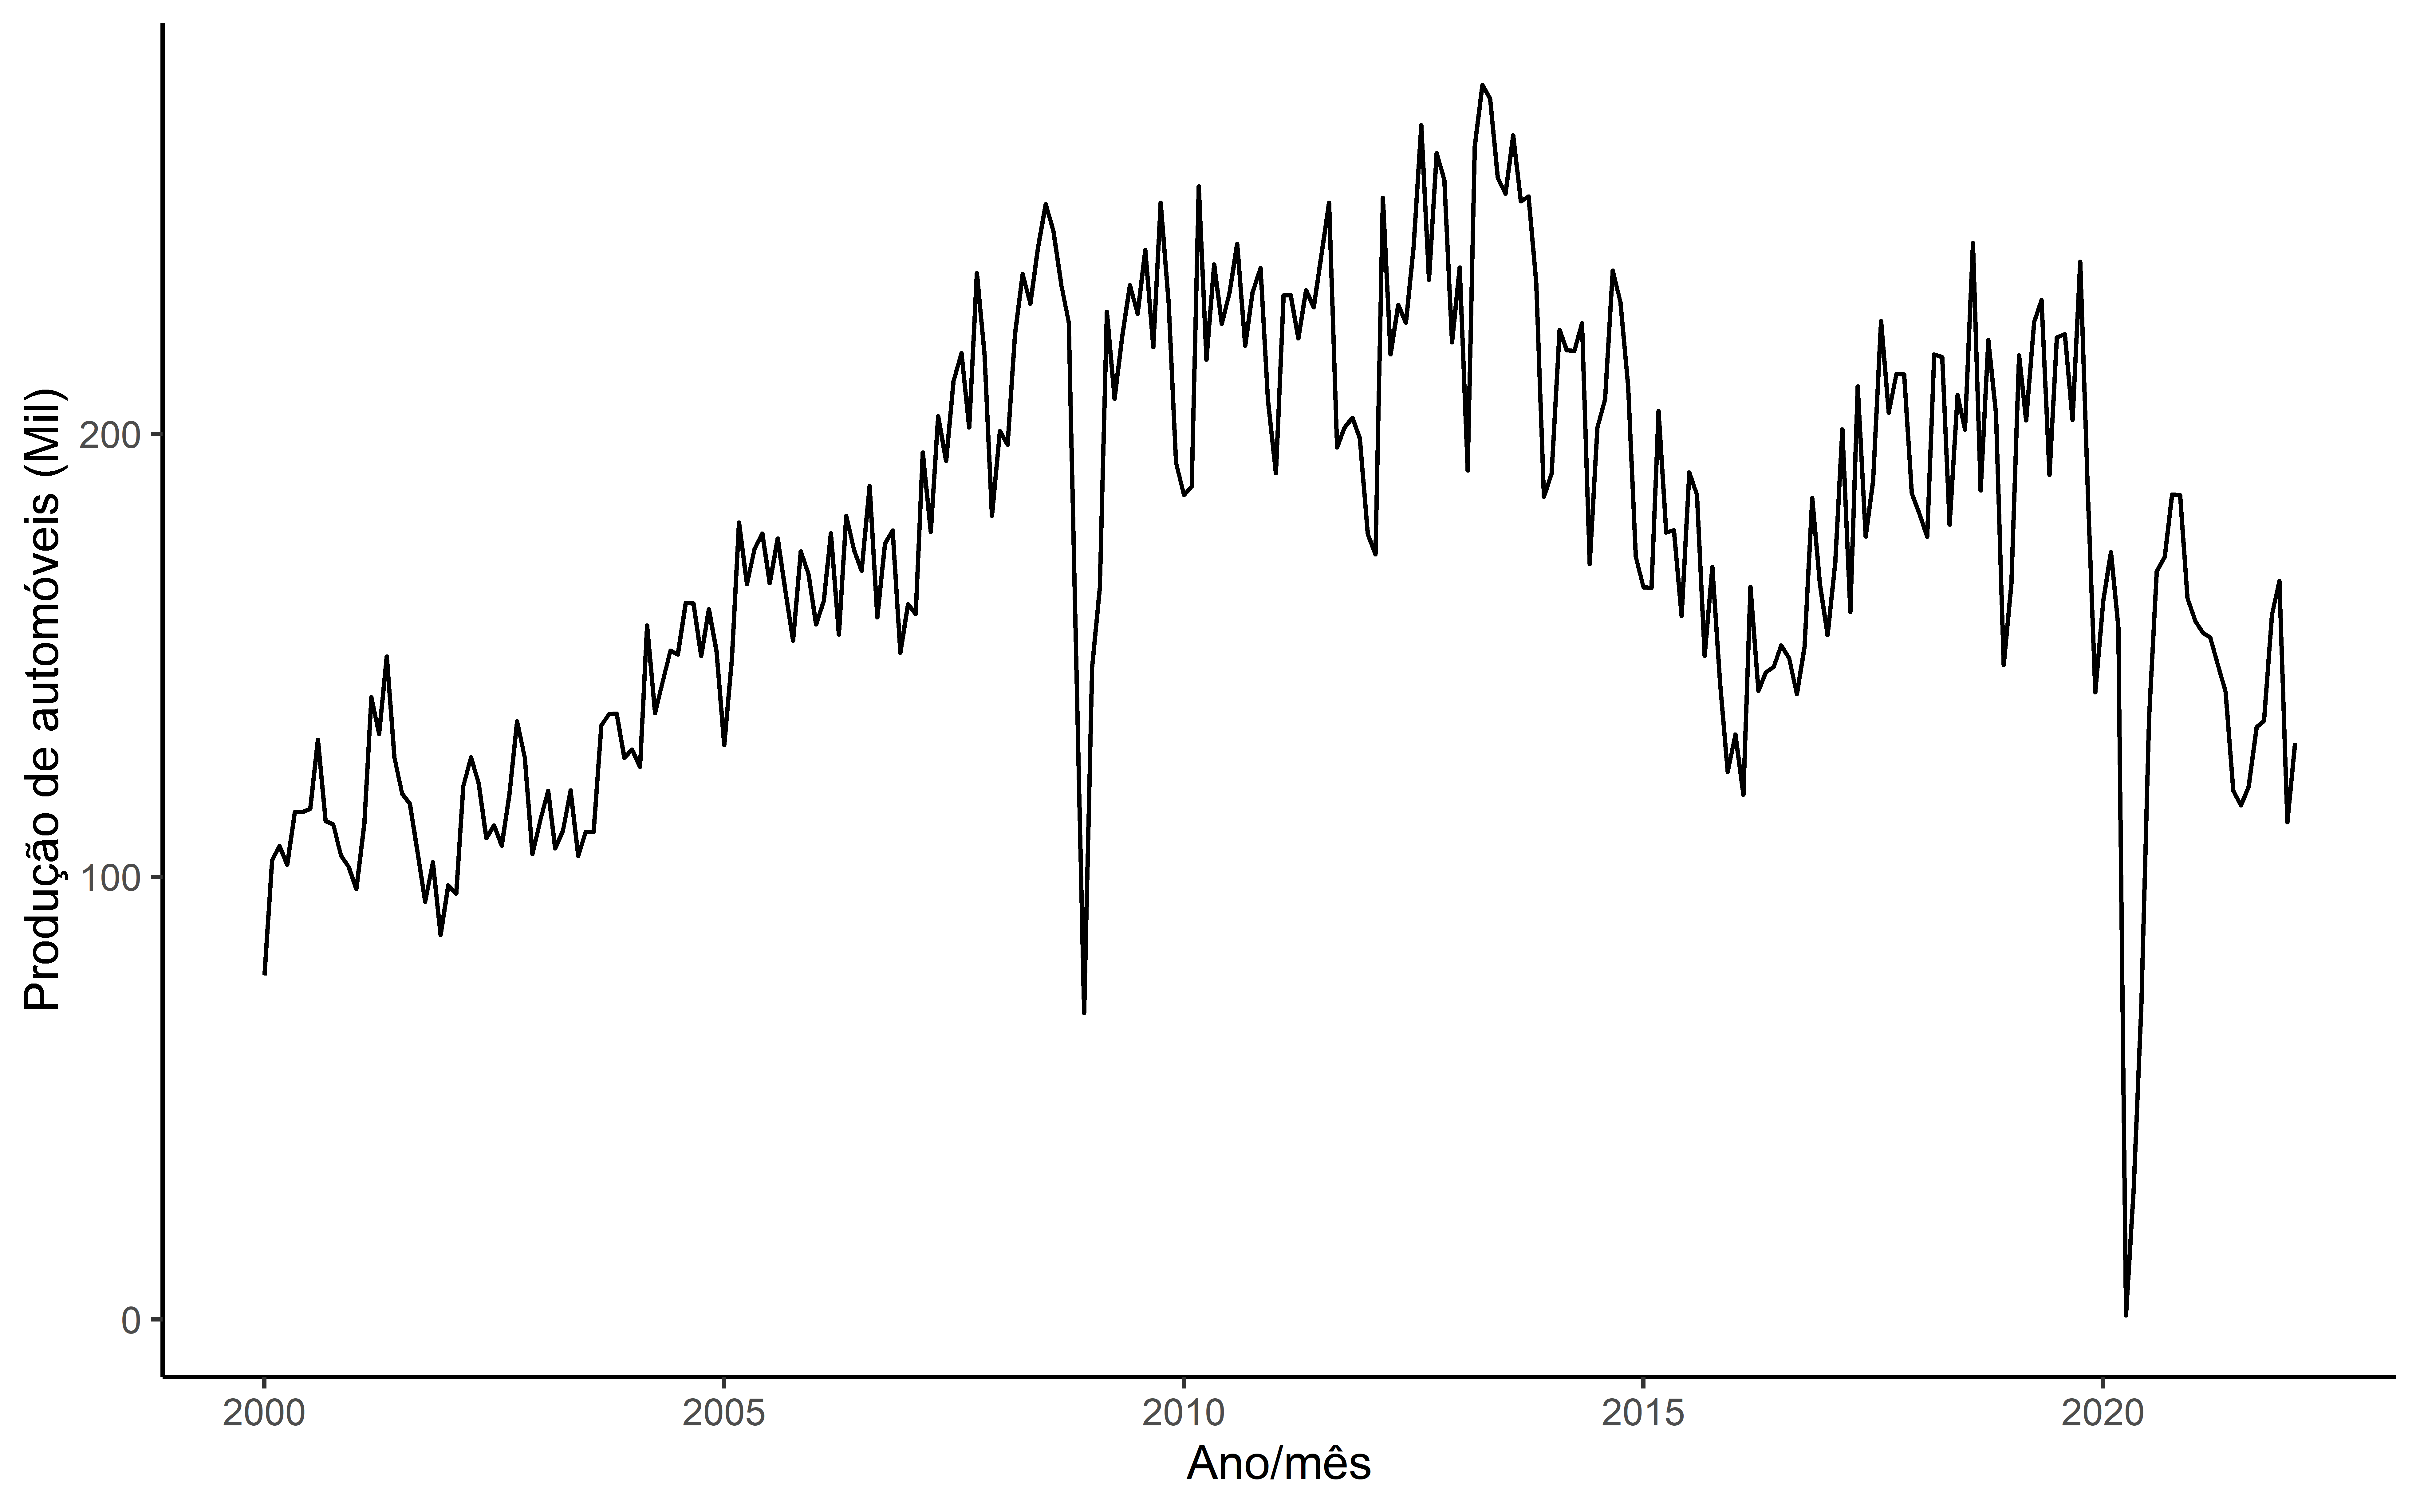
\includegraphics[width=0.8\textwidth]{figuras/automovel graph.png}
    \caption{Produção de automóveis (2000-2022)}
    \label{fig:graph}
\end{figure}

Um ponto importante apresentado no \autoref{fig:graph} descreve as quebras estruturais apresentadas na série. A base para estimar quebras em modelos de regressão de séries temporais foi dada por \citeonline{bai1994least} e expandida para quebras múltiplas por \citeonline{bai1997estimating} e \citeonline{bai1998estimating}. O teste utilizado utiliza o mesmo algoritmo descrito em \citeonline{bai2003computation} para estimação simultânea de múltiplas quebras estruturais. \autoref{tab:04} apresenta o resultado do teste indicando que entre 2000 e 2022 há cinco quebras estruturais. A partir do teste, a periodicidade mensal dos dados foi restringida para cobrir o período entre janeiro de 2015 e fevereiro de 2022 e assim, tornar as estimativas mais precisas e sem problemas de quebra estrutural.

\begin{table}[H] 
  \centering
  \caption{Teste de múltiplas quebras estruturais}
    \begin{tabular}{l|ccc}
    \hline
    Quebra estrutural &  Intervalo inferior & Período & Intervalo superior \\
    \hline
    1 & Nov/2003  & Jan/2004  & Fev/2004 \\
    2 & Out/2006  & Mar/2007  & Abr/2007  \\
    3 & Dez/2007  & Jul/2010  & Ago/2015  \\
    4 & Jul/2014  & Nov/2014  & Mar/2015  \\
    5 & Nov/2012  & Nov/2018  & Abr/2020  \\
    \hline
    \multicolumn{4}{l}{Elaboração própria.}
    \end{tabular}%
  \label{tab:04}%
\end{table}%

Para alguns dos experimentos, a ocorrência de não linearidade dos dados pode acarretar em problemas nas estimativas. Para isso, também foi verificado os testes de \citeonline{tsay1986nonlinearity} e \citeonline{chan1991percentage} para verificar se há ou não a presença de não linearidade nos dados. A \autoref{tab:05} mostra pelo teste que os dados aceitam a hipótese nula de presença de não linearidade nos dados apresentados.

\begin{table}[H] 
  \centering
  \caption{Testes de não linearidade}
    \begin{tabular}{l|ccl}
    \hline
    Teste & Valor & p-valor & Hipótese nula  \\
    \hline
    T'say's & 2,04  & 0,00 & \multicolumn{1}{m{15em}}{A série temporal segue algum processo auto regressivo}  \\
    \multicolumn{1}{m{15em}|}{Razão verossimilhança para não linearidade de limiar} & 33,4 & 0,03 &  \multicolumn{1}{m{15em}}{A série temporal segue algum processo auto regressivo} \\
    \hline
    \multicolumn{3}{l}{Elaboração própria.}
    \end{tabular}%
  \label{tab:05}%
\end{table}%

% para o período entre janeiro de 2015 e fevereiro de 2020. A periodicidade dos dados foi escolhida por três motivos, primeiro, mesmo que os dados de produção de automóveis tenham informações dos anos 50 até os dias atuais, o cenário histórico brasileiro apresenta muita distorção (por exemplo, hiper inflação) capazes de gerar viés nas estimativas de previsão e dos anos 2000 em diante os dados estão mais suavizados sujeitos a menos choques. Em segundo lugar, a maioria das variáveis explicativas não possuem informações muito antigas, sendo disponibilizadas apenas após os anos 2000. Por último, os dados apresentam diversos pontos de quebra estruturais, o que pode gerar vieses nas estimativas de previsão. Por isso, recortamos a série dos dados de acordo com a última quebra apresentada.

A partir das especificações da plataforma e da literatura, foram inclusos controles de sazonalidade, fluxo médio de carros em área de pedágio (\textit{proxy} para o fluxo de carros), taxa de câmbio, produção industrial, PIB, taxa de câmbio, taxa de juros \textit{ex ante} e os preços do combustível, etanol e dieesel. Todas as variáveis foram transformaras em logaritmo natural para suavizar os valores. No caso do número de automóveis, por exemplo, a aplicação do logaritmo natural permite variação menor entre os meses. Também foi incluído a defasagem de até 3 meses nas variáveis dos preços e taxa de juros e foi incluída as variáveis de fluxo de carro em área de pedágio em até 3 meses na frente.

Separamos também as estimativas em 4 grupos de exclusão. O primeiro representa os preço e suas defasagens, o segundo foram os juros e suas defasagens, o terceiro foram o PIB e a produção industrial e o último foi a variável de fluxo de carro e seus valores futuros. Cada grupo foi selecionado com o objetivo de evitar problemas de colinearidades entre as variáveis. A presença de colinearidade entre as variáveis pode gerar erro na interpretação dos coeficientes. Com a finalidade de evitar esse problema, os modelos estimados são programados para estimar essas variáveis de forma separada.

A plataforma permite projetar linearmente as variáveis explicativas para que seja possível prever a produção de automóveis. Os testes de validação cruzada foram realizados numa seleção de 10 janelas utilizando a mediana como medida de mensuração e com o horizonte de previsão para 12 meses. A mediana foi escolhida neste caso devido aos dados apresentarem casos de \textit{outliers}\footnote{Como mostra a \autoref{fig:graph} os \textit{outliers} apresentados fazem com que a média possa causar medidas errôneas sobre os testes, tornando a mediana um parâmetro mais preciso.} aparentes no período de validação cruzada. O horizonte de previsão foi selecionado com o intuito de obter resultados de médio prazo, uma vez que o objetivo da previsão é projetar 22 meses a frente.

Como mostra a \autoref{fig:04}, os 20 modelos que apresentaram a melhor acuraria, com o menor Erro Percentual Absoluto Médio (MAPE), foram os modelos de \textit{Forecast Combination} e ARIMA. Seguindo o ranqueamento do gráfico, é possível afirmar que projetando os próximos 22 meses, o melhor modelo erra 8,26\%, enquanto que o 20º melhor modelo erra 12,7\%.

\begin{figure}[H]
    \centering
    \caption{Resultado dos 20 melhores modelos}
    \includegraphics[width=1\textwidth]{figuras/geral.png}
    \begin{flushleft}
    Fonte: Elaboração própria.
    \end{flushleft}
    \label{fig:04}
\end{figure}

Seguindo o mesmo raciocínio, a \autoref{fig:05} apresenta graficamente a série do total de automóveis produzidos mensalmente a previsão até dezembro de 2023 de acordo com os 10 melhores modelos indicados na \autoref{fig:04}. Como mostra o \autoref{fig:05}, em 2023, a tendência é que o número de produção de automóvel seja maior que 2021 e 2022 e atinga em dezembro, uma produção de cerca de 197 mil automóveis. Mesmo que seja em passos lentos, a expectativa é que aos poucos, o mercado se recupere da grande baixa de produção de automóveis ocorrida em 2020 e 2021 (devido a pandemia da covid-19) e que aos poucos o cenário seja mais favorável. O gráfico também mostra que o cenário é diverso, a depender do modelo especificado. Dentre os 20 melhores, o modelo 7 foi o mais pessimista e o modelo 1 o mais otimista

\begin{figure}[H]
    \centering
    \caption{Valores previstos para os 10 melhores modelos}
    \includegraphics[width=1\textwidth]{figuras/previsao.png}
    \begin{flushleft}
    Fonte: Elaboração própria.
    \end{flushleft}
    \label{fig:05}
\end{figure}

\subsection{Forecast Combination}

O modelo \textit{Forecast Combination} que apresentou a melhor acurácia combina 10 modelos utilizando uma Regressão de Mínimos Quadrados Restrita. Observando de forma geral o comportamento do modelo, os valores preditos tem tendência semelhante ao que se apresenta o valor verdadeiro, indicando consistência nas estimações. No teste de validação cruzada, O MAPE consegue indicar que há certa consistência entre as janelas de teste. Contudo, este modelo não é capaz de testar os parâmetros para as variáveis explicativas que tornam capazes de interpretar os coeficientes. O modelo também não disponibiliza testes que verificam o erro e tornam o resultado previsto mais robusto. Para realizar esses testes foi avaliado os modelos ARIMA em busca do modelo mais consistente.

%\begin{figure}[H]
%    \centering
%    \includegraphics[width=1\textwidth]{figuras/fc_2.png}
%    \caption{Comparação de curva original com a predita - Forecast Combination}
%    \label{fig:06}
%\end{figure}






\subsection{ARIMA}

Diferente do modelo de \textit{Forecast Combination}, o ARIMA é um modelo econométrico muito utilizado em séries temporais com o objetivo de gerar previsão. Em grande parte, os modelos ARIMA partem de pressupostos que podem ser testados a partir da análise dos resíduos e avaliação de correlação temporal.

% O molhor modelo foi ARIMA(0,0,0)

%\begin{table}[H] 
%  \centering
%  \caption{Informações gerais do modelo - ARIMA}
%    \begin{tabular}{l|cccc}
%    \hline
%    Teste & MAPE & WMAPE & MPE &  RMSE \\
%    \hline
%    Valor & 311.88 & 20.81  & -304.3  & 37428.69   \\
%    \hline
%    \end{tabular}%
%  \label{tab:05}%
%\end{table}%

% Ao observar o gráfico acima (Figura 3), percebe-se uma correlação significativa no lag1, com um padrão seguido a cada 5 defasagens além de incluir a afirmação da possibilidade de uma série não estacionária, o motivo que leva a isso é sua defasagem não cair abruptamente para zero. Nota-se também uma variação, representando um caráter sazonal. Além disso, repara-se uma autoregressividade exponencial nos pontos relatados. Dessa forma, há uma alternativa de ser um modelo AR.



%Na \autoref{fig:10}

%\begin{figure}[H]
%    \centering
%    \includegraphics[width=1\textwidth]{figuras/arima_3.png}
%    \caption{Comparação de curva original com a predita - ARIMA}
%    \label{fig:10}
%\end{figure}

A \autoref{fig:11} descreve as variáveis utilizadas em cada um dos 20 melhores modelos (começando do melhor modelo, a esquerda). A ordem das covariadas é definida pela magnitude do coeficiente de cada uma das variáveis explicativas. A ordem de significância estatística vai do azul escuro, como as variáveis mais significantes, até o vermelho escuro, que são as variáveis de menos significância estatística. De acordo com as estimativas, a variável \textit{$fs_pim$} (Produção industrial) foi a que teve maior efeito e também foi bastante significativa em qualquer um dos modelos. Em um horizonte futuro, o modelo 1 nos diz que um aumento de 1\% na produção industrial é capaz de aumentar em 3,2\% a produção de automóvel. O PIB, por ser uma variável de exclusão em relação a produção industrial, apareceu em poucos modelos, também indicando sinal positivo.

Como \textit{proxy} de fluxo de automóveis, o indicador de número de carros que atravessam um trecho rodoviário com pedágio teve efeito positivo, indicando que o maior fluxo de carros ocasiona uma maior produção de automóveis. As variáveis de taxa de câmbio e de juros apresentaram sinal negativo, indicando que uma desvalorização cambial e um aumento no custo de empréstimo gera uma redução na produção de carros. Essas variáveis foram significativas em poucos modelos. Esses efeitos vão todos no mesmo sentido proposto pela literatura que avalia os efeitos macroeconômicos na produção de automóvel \cite{ramey2004tracking,nawi2013determinants,muhammad2013relationship,verissimo2015desempenho,islam2016analysis}. Por último, a variável de preços do etanol não foi significante estatisticamente, enquanto que o preço do diesel nos dois meses anteriores foi negativamente relacionado com a produção de automóvel. 

Esse resultado é capaz de ir mais além: a partir do cenário macroeconômico é possível gerar situações mais otimistas ou pessimistas sobre a previsão na produção de automóveis. Por exemplo, como foi exemplificado no quesito anterior, a guerra entre a Rússia e Ucrânia pode acarretar numa grande fuga de capital estrangeiro da Rússia em busca de outro país emergente participante do BRICS. Na ocorrência deste efeito, o país pode apresentar uma tendência de maior produção automobilista, uma vez que a entrada de capital estrangeiro afetará o câmbio.

\begin{figure}[H]
    \centering
    \caption{Significância e peso das variáveis inclusas no modelo - ARIMA}
    \includegraphics[width=1\textwidth]{figuras/variaveis.png}
    \begin{flushleft}
    Fonte: Elaboração própria.
    \end{flushleft}
    \label{fig:11}
\end{figure}

No geral, mesmo que o modelo 1 da \autoref{fig:11} apresente a melhor acurácia no MAPE (11,2\%), as variáveis selecionadas não são capazes de responder com precisão os determinantes para a produção automobilística. Por isso, o modelo selecionado para avaliar foi o modelo 2. Contudo, é preciso realizar outros testes para validar a real consistência deste modelo.

Na \autoref{fig:graph}, não há possibilidade clara de distinguir se a série apresenta ou não estacionariedade, pois a mesma apresenta variações em alguns intervalos de tempo, o que não torna tão claro se a série é de fato estacionária. Diante disso, verifica-se a comparação dos correlogramas FAC com o objetivo de identificar a tendência, sazonalidade, assim como a filtragem de resíduos. O teste de função autocorrelação (ACF) projeta as defasagens do resíduo da estimação e testa se existe correlação nas defasagens do erro. As barras azuis representam as bandas de erro. Qualquer reta que fica entre as barras laranjas são não significantes estatisticamente. Em outras palavras, qualquer valor de correlação fora dessa área possuem grandes chances de ter uma correlação e não um acaso estatístico. O gráfico de autocorrelação residual define por padrão um intervalo de confiança de 95\%. Como mostra a \autoref{fig:08}, a série possui correlação residual nos primeiras defasagens, o que torna as estimativas de previsão duvidosas.

\begin{figure}[H]
    \centering
    \caption{Resultado do teste ACF}
    \includegraphics[width=1\textwidth]{figuras/ACF.png}
    \begin{flushleft}
    Fonte: Elaboração própria.
    \end{flushleft}

    \label{fig:08}
\end{figure}

Desta forma, o modelo 7 aparece como resultado mais consistente. Além de não apresentar nenhuma autocorrelação residual no teste ACF, a distribuição do erro apresenta comportamento normal. O modelo apresenta uma especificação ARIMA (1,0,2), com MAPE de 13\%. O último teste para verificação deste modelo é a validação cruzada, considerada uma técnica utilizada para avaliar a capacidade de generalização de um conjunto de dados independente. A \autoref{fig:07} apresenta o resultado do MAPE e RMSE agregado para cada janela de teste de validação cruzada. Os vários testes em janelas periódicas diferentes não mostram diferenças significativas no MAPE e RMSE, mantendo uma acuraria semelhante ao que apresentamos no modelo de previsão geral. Dessa forma, nossos resultados não parecem cair no problema de \textit{Under-fitting/Over-fitting} ou não parecem ser mal generalizados.

\begin{figure}[H]
         \centering
        \caption{Resultado de todas as janelas da validação cruzada ARIMA}
         \includegraphics[width=1\textwidth]{figuras/validacao_cruzada.png}
         %\label{fig:three sin x}
    \begin{flushleft}
    Fonte: Elaboração própria.
    \end{flushleft}

        \label{fig:07}
\end{figure}

Após os testes e a comprovação de que o modelo 7 é de fato o mais consistente, a \autoref{fig:09} apresenta graficamente a previsão deste modelo até dezembro de 2023. Os indicativos mostram que em 2022 o setor de automóvel irá ter uma queda na produção de automóveis (-11,2\%), mas em 2023 esse valor pode crescer 6,41\%. É possível que em 2022 o cenário seja mais pessimista mesmo que o câmbio apresenta sinais favoráveis, pois, como foi indicado na questão anterior, a guerra entre a Rússia e a Ucrânia afeta o mercado brasileiro não apenas pelo lado das \textit{commodities}, mas também afeta o setor automobilístico com a falta de paládio, um insumo importante na produção de automóveis. A expectativa é que após a guerra, o comportamento na produção seja mais estável, indicando que após um período de queda devido a crise da covid-19 e a guerra da Ucrânia e Rússia, o setor automobilístico pode um período mais instável de produção.

%Antes, em 2016 também teve um período de baixa produção). Em 2021 o Brasil produziu em média 170 mil automóveis por mês. Como mostra o gráfico, a tendência é de uma elevação no mês de maio e dezembro na produção de automóveis e uma redução nos três meses seguintes. Em 2023 a tendência é que o número de produção de automóvel seja maior que 2021 e 2022 e atinga em dezembro, uma produção de cerca de 197 mil automóveis. Mesmo que seja em passos lentos, a expectativa é que aos poucos, o mercado se recupere da grande baixa de produção de automóveis ocorrida em 2020 e 2021 (devido a pandemia da covid-19) e que aos poucos o cenário seja mais favorável.


\begin{figure}[H]
    \centering
    \caption{Resultado da previsão o modelo 7 - ARIMA}
    \includegraphics[width=1\textwidth]{figuras/previsao_arima.png}
    \begin{flushleft}
    Fonte: Elaboração própria.
    \end{flushleft}
    \label{fig:09}
\end{figure}

\newpage
%\bibliographystyle{abnt}
\bibliography{Referensi}
\end{document}